\chapter{Logistic Regression}
\label{chapter:logistic}
\begin{center}
  {\Large\textit{The purpose of computing is insight, not numbers.\\- Richard Hamming}}
\end{center}
\vspace{0.2in}

\section{Formulation}

\emph{Logistic regression} is probably familiar to many of you, so we will try to formulate the problem from a few different angles.  

\subsection{Presenter's viewpoint}
Let's consider the viewpoint of a data scientist explaining logistic regression to a non-technical audience.  One challenge is that the dependent variable in the training data does not explicitly coincide with the model output.  For example, consider the data set \T{training.csv},

\begin{minted}{bash}
  age,dosage,recovers
  33,100,1
  22,90,0
  15,90,1
  23,85,0
\end{minted}

The variable in the column \T{recovers} is one when the subject recovers from cancer, and zero when they do not.  \T{dosage} is the dosage of some hypothetical drug.  A logistic regression could be used to take in age and dosage, and output the probability that the subject recovers.  In this case, our model output could look like

\begin{minted}{bash}
  age,dosage,prob_recovers
  33,100,0.85
  22,90,0.6
  15,90,0.7
  23,85,0.4
\end{minted}

So our model output is a probability $p\in[0,1]$, which does not match up with our dependent variable.  This is in contrast to the use of logistic regression for \emph{classification}.  Here for example, a cutoff is chosen such that if \T{prob\_recovers} $ > $ \T{cutoff}, then we classify the subject one that will recover.  If \T{cutoff} = 0.5, then out model output would be $(1, 1, 1, 0)$, which could be compared directly with the training data, as is the case with linear regression.

\subsection{Classical viewpoint}
The classic formulation of logistic regression starts with assumptions about the probability of $y$ taking either 0 or 1, given the value of $x$.  Let's write this as $\rmP[y=0\g x]$ and $\rmP[y=1\g x]$.  The assumption is
\begin{align}
  \log\left[ \frac{\rmP[y = 1\g x]}{1 - \rmP[y=1\g x]} \right] &=x \cdot w.
  \label{logistic:align:basic-assumption-1}
\end{align}
This can be re-written using the \emph{logit} function, defined by $\logit z := \log[z / (1-z)]$.  Solving for $\rmP[y=1\g x]$ we arrive at
\begin{align}
  \rmP[y=1\g x] &= \frac{e^{x\cdot w}}{1 + e^{x\cdot w}}.
  \label{logistic:align:basic-assumption-2}
\end{align}
This can also be re-written using the \emph{logistic sigmoid} function $\sigma(z) := \exp(z)/(1 + \exp(z))$.  In other words, our model assumes $\rmP[y=1\g x] = \sigma(x\cdot w)$.  This function has the nice property that it takes values in the interval $[0,1]$, as a probability should.  Moreover, it behaves nicely when differentiated (see exercise \ref{logistic:exercise:sigmoid}).
\begin{figure}
  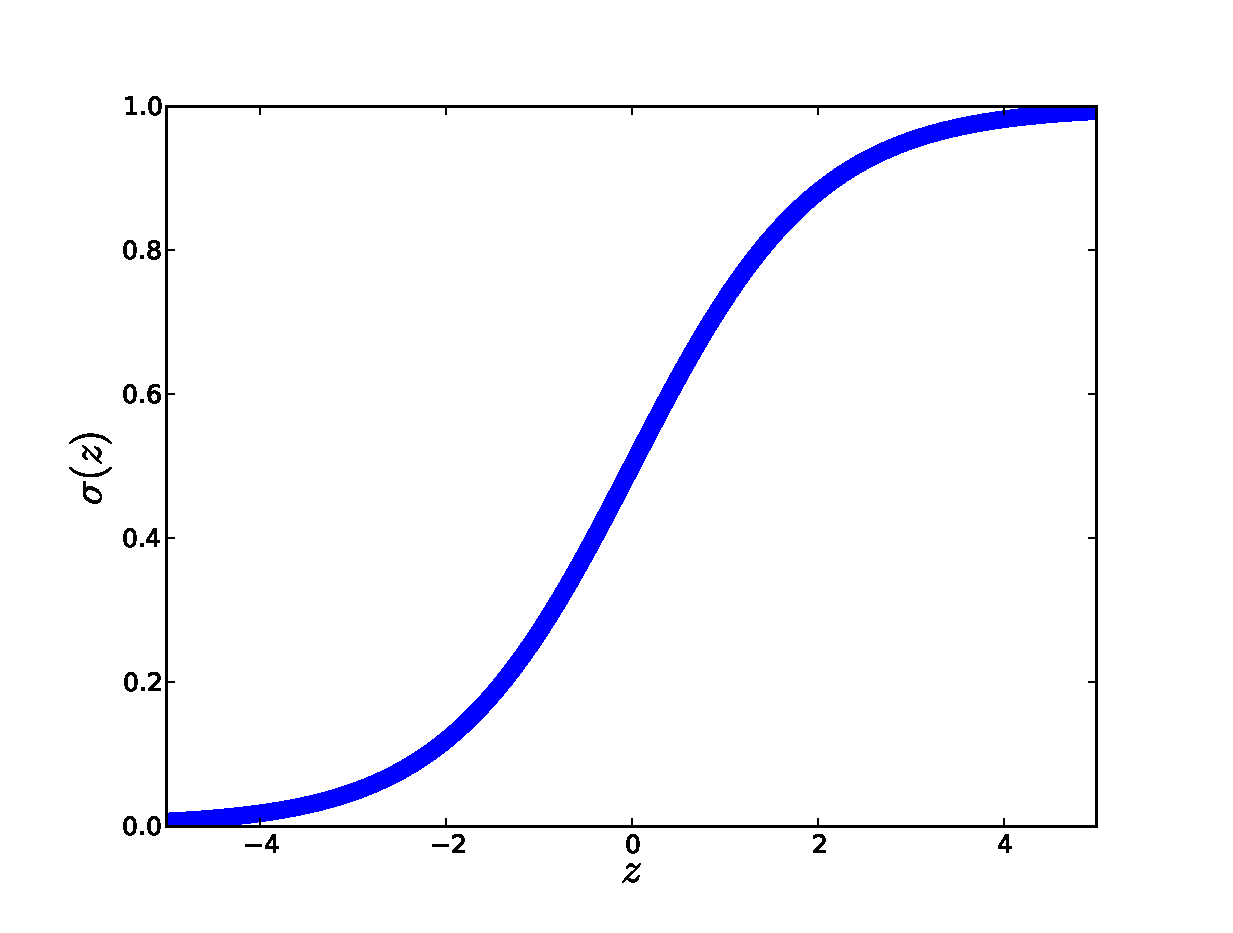
\includegraphics[width=0.7\textwidth]{../images/sigmoid}
  \caption{Plot of the sigmoid function $\sigma(z)$ from for $z\cdot w\in[-5, 5]$.}
\end{figure}

\begin{exercise}
  Show that \eqref{logistic:align:basic-assumption-1} implies \eqref{logistic:align:basic-assumption-2}.
\end{exercise}

\begin{exercise}
  \label{logistic:exercise:sigmoid}
  Show that $\sigma'(z) = \sigma(z)(1 - \sigma(z))$, and $\sigma(-z) = 1 - \sigma(z)$.
\end{exercise}

\subsection{Data generating viewpoint}
\label{logistic:subsection:data-generating-viewpoint}
One can devise a data generating process that gives rise to the classical viewpoint.  Suppose we have a latent variable $z$ such that our observed variable $y$ is given by $y := \one_{z>0}$.  For example, $y=1$ could indicate ``patient recovers from cancer'', and $z$ is the health level of the patient.  To tie this to independent variables we consider the model
\begin{align*}
  z &= x\cdot w + \eps,
\end{align*}
where $\eps$ is a random variable with probability density $\sigma'(z) = \sigma(z)(1 - \sigma(z))$ (see exercise \ref{logistic:exercise:sigmoid}).  This implies
\begin{align*}
  \rmP[y = 1] &= \rmP[z > 0] = \rmP[\eps > -x\cdot w] = \int_{-x\cdot w}^\infty \sigma'(\eta)\d\eta = \int_{-\infty}^{x\cdot w}\sigma'(\eta)\d\eta\\
  &= \sigma(x\cdot w),
\end{align*}
where the second to last equality is justified by verifying $\sigma'(z) = \sigma'(-z)$.  In other words, $y$ has probability mass function given by \eqref{logistic:align:basic-assumption-2}.

This formulation is useful because it allows one to explore questions of model error.  For example, suppose $\eps$ depends on $x$.  This could arise if there is error in some of the labels, and this error depends on $x$ (suppose it is more difficult to determine recovery in older patients).  More generally, $\eps$ represents the deviation of the latent variable $z$ from our modeled value $x\cdot w$.  Re-phrasing our conversation at the beginning of chapter \ref{chapter:linear}, there is no need to assume that the world is fundamentally random.  There exists some set of variables $(x, v)$ that tell us with certainty whether or not a person will recover (for example, the position and state of every particle in the universe).  It just happens that in our data set we do not have access to all of them (we only have $x$), or to the correct functional form of their relationship to the observed variable $\one_{z>0}$.  If there true form is $z = f(x, v)$, we can write
\begin{align}
  \label{logistic:align:model-error}
  z &= x\cdot w + \eps,\quad \mbox{ where }\quad\eps := x\cdot w - f(x,v).
\end{align}
In other words, $\eps$ represents the uncertainty in our model.


\begin{exercise}
  Referring to the paragraph above \eqref{logistic:align:model-error}, restate the issue of mislabeled data as a problem of modeling error.
\end{exercise}


\section{Determining the regression coefficient $w$}
Before we proceed, we should define a couple things.  A matrix $A$ is said to be \emph{positive definite} if it is symmetric and all of its eigenvalues are positive.  Rather than computing the eigenvalues, one can check that, for every nonzero vector $v$, $v^TAv>0$.  A function $f(w)$ is strictly convex if, for all $\lambda\in[0,1]$, and points $w^1, w^2\in\RK$, $f(\lambda w_1 + (1-\lambda)w_2) < \lambda f(w_1) + (1-\lambda)f(w_2)$.  If $f$ has two continuous derivatives, then, rather than checking the above inequality, one can check that the hessian matrix $\nabla^2f(w)$ is positive definite at every point $w\in\RK$.  If a function $f:\RK\to\Rone$ is strictly convex, then any local minimum is also the global minimum.  Note that it is possible for the function to not have any minimum (e.g. it can keep getting smaller and smaller as $w\to\infty$).  This is very important for optimization, since most algorithms are able to find local minimums, but have a hard time verifying that this is a global minimum.

The coefficient $w$ in \eqref{logistic:align:basic-assumption-1}, \eqref{logistic:align:basic-assumption-2} is usually determined by maximum likelihood, although a Bayesian approach may be used.  In either case, we need the likelihood.  Recalling the notation of chapter \ref{chapter:notation}, the likelihood is
\begin{align*}
  p(Y\g w) &= \prod_{n=1}^N p(Y_n\g w) = \prod_{n=1}^N \rmP[y=1\g x=X_{n:}, w]^{Y_n}\rmP[y=0\g x=X_{n:},w]^{1-Y_n}\\
  &= \prod_{n=1}^N \sigma(X_{n:}\cdot w)^{Y_n}(1-\sigma(X_{n:}\cdot w))^{1-Y_n}.
\end{align*}
This can be checked by considering the cases $Y_n=0$ and $Y_n=1$ separately.  The maximum likelihood solution is the point $w_{ML}$ that maximizes this.  Instead we usually minimize the negative log likelihood, that is
\begin{align}
  \label{logistic:align:ML-soln}
  \begin{split}
    w_{ML} :&= \arg\min_w L(w),\qquad\mbox{where,}\\
    L(w) :&= -\sum_{n=1}^N\left[ Y_n\log\sigma(X_{n:}\cdot w) + (1-Y_n)\log(1-\sigma(X_{n:}\cdot w)) \right].
  \end{split}
\end{align}
Note that $L(w)$ will always be non-negative since $\sigma\in(0, 1)$.
Since $\sigma'(z) = \sigma(z)(1-\sigma(z))$, we find that
\begin{align*}
  \frac{\p L}{\p w_k} &= \sum_{n=1}^N\left[ \sigma(X_{n:}\cdot w) - Y_n \right]X_{nk},\qquad
  \frac{\p^2 L}{\p w_k w_j} = \sum_{n=1}^N\sigma(X_{n:}\cdot w)(1 - \sigma(X_{n:}\cdot w)) X_{nk}X_{nj}.
\end{align*}
Or, with $\nabla L$ and $\nabla^2L$ denoting the gradient and hessian matrix (the matrix with $kj$ entry equal to $\p^2L/\p w_k\p w_j$),
\begin{align}
  \label{logistic:align:grad-hess}
  \begin{split}
    \nabla L(w) &= \sum_{n=1}^N\left[ \sigma(X_{n:}\cdot w) - Y_n \right]X_{n:},\\
    \nabla^2L(w) &= \sum_{n=1}^N\sigma(X_{n:}\cdot w)(1 - \sigma(X_{n:}\cdot w)) X_{n:}^TX_{n:}.
  \end{split}
\end{align}
One can check that for any vector $v\in\RK$,
\begin{align*}
  v\cdot\nabla^2L(w)v &= \sum_{n=1}^N(v\cdot X_{n:})^2\sigma(X_{n:}\cdot w)(1-\sigma(X_{n:}\cdot w)),
\end{align*}
which is greater than or equal to zero, and strictly greater than zero for all vectors provided the matrix $X$ has rank $K$.  In other words, if the data columns are linearly independent, then the hessian is positive definite for every $w$, and hence the function $L$ is strictly convex.  This implies that any local minimum of $L$ is a global min, which can be shown to be $w_{true}$ in the limit $N\to\infty$ if the rows $X_{n:}$ are statistically independent samples and the data generating process is as described in section \ref{logistic:subsection:data-generating-viewpoint} with $w=w_{true}$.  To make this last statement plausible, note that in this ideal case, the expected value of $\nabla L(w)$ is $\sum_n\left[ \sigma(X_{n:}\cdot w) - \sigma(X_{n:}\cdot w_{true}) \right]$, of which $w=w_{true}$ is the minimizing value.  Since $\nabla L(w)$ is a sum of random variables, we can rescale it by $1/N$ and see that it should approach its expectation.  

\begin{exercise}
  Show that for fixed $w$, $\nabla^2L(w)$ is positive definite for all $w$ if and only if $X$ has rank $K$.
\end{exercise}

\begin{digression*}[Don't truncate linear regression!]
  Suppose we are told to determine the probability that a customer will keep their membership with ``Super Fitness Gym'' for longer than one year.  We ask the general manager for data and she gives us height, weight, age, and \emph{length of gym membership in months} for 10,000 customers (ignore the fact that some customers have only been there less than a year and have not had the chance to be there a full year).  Now we have membership information as a semi-continuous variable \emph{membership-length}$ = 1,2,\dots$, but we are asked to predict a binary outcome (either Yes or No).  One approach would be to set $Y = 1$ if membership length is greater than 12, and 0 if it is less.  However, this approach throws out information about how long someone has been at the gym.  For example, people who quit in 1 month are treated the same as those who quit in 11.  A better approach would probably be to use a linear regression model where we try to predict the number of months that the membership will last.  To turn this into a probability, we would use a Bayesian approach to determine $p(y\g x, Y)$ as in section \ref{linear:subsection:generic} equation \eqref{linear:align:predictive}.  Since the data is discrete but ordered (1,2,3,\ldots) a better approach would be so called \emph{ordinal regression}.  Since some people have not quit (hence we don't know how long they will be there) the best approach would be \emph{right-censored ordinal regression}.
\end{digression*}

The Bayesian approach proceeds as in chapter \ref{chapter:linear}.  That is, we choose a prior $p(w)$ and form the posterior $p(w\g Y)\propto p(w)p(Y\g w)$.  Gaussian priors are common.  Also common is the Laplace prior $p(w)\propto \exp\left\{ -\alpha\|w\|_1 \right\}$, where $\|w\|_1 = \sum |w_k|$ is the L1 norm of $w$.  See section \ref{logistic:section:L1}.

\begin{exercise}
  Sometimes, otherwise well-meaning individuals, use linear regression to solve a logistic regression problem.  Consider the case of spam filtering.  Your independent variables are the num ber of times certain words appear in the document.  For example, the word ``V1@Gra'' is one of them, and of course this world is almost always associated with spam.  You are told to produce a model that gives the probability that an email is spam.  Your colleague, Randolph Duke, tells you that since the dependent variable $y$ is a number (in this case 0 or 1), he will build a linear regression that takes in $x$ and tries to predict $y$.  Of course the result won't be in the interval $[0, 1]$, but, \underline{after training}, he will truncate it, or re-scale it, so that it is.  What is wrong with Mr. Duke's approach?
\end{exercise}


\begin{exercise}[Heteroscedastic probit models]
  A \emph{probit regression} is just like a logistic regression, but rather than the logistic sigmoid $\sigma(x\cdot w)$, we use the Gaussian cumulative distribution function $\Phi(x\cdot w)$. 
  \begin{enumerate}
    \item Following the reasoning in section \ref{logistic:subsection:data-generating-viewpoint}, show that if $y = \one_{z>0}$ with $z = x\cdot w_{true}+\eps$ with $\eps\sim\calN(0, \lambda^2)$ being \iid, then  $\rmP[y=1\g x] = \Phi(x\cdot w_{true}/\lambda)$.
    \item If we perform a probit regression, we will assume $\rmP[y=1\g x] = \Phi(x\cdot w)$.  In other words, we will set $\lambda=1$.  From the standpoint of building a model that takes in $x$ and spits out $\rmP[y=1\g x]$, why doesn't the assumption $\lambda=1$ matter?
    \item Suppose now that $\eps \sim\calN(0, (x\cdot v_{true})^2)$.  Show that our model should be
      \begin{align*}
        \rmP[y=1\g x] &= \Phi\left( \frac{x\cdot w}{x\cdot v} \right).
      \end{align*}
    \item Using the notation
      \begin{align*}
        \Phi_n :&= \Phi\left( \frac{X_{n:}\cdot w}{X_{n:}\cdot v} \right),
      \end{align*}
      write down the likelihood and negative log likelihood associated to the independent variable matrix $X$ and dependent variable vector $Y$.
  \end{enumerate} 
  Minimizing the negative log likelihood is obviously more difficult because it involves a nonlinear combination of variables.  For that reason, an iterative technique is used, whereby $v$ is fixed and the minimum over $w$ is obtained, then $w$ is fixed and a minimum over $v$ is obtained.  This iterative procedure is repeated until the negative log likelihood stops changing very much.
\end{exercise}

\section{Multinomial logistic regression}
\label{logistic:section:multinomial}
Logistic regression can be generalized to the case where $y$ takes on a number of values.  Call each of these classes $C_m$ for $m=1,\cdots,M$.  We can generalize \eqref{logistic:align:basic-assumption-1} to get
\begin{align*}
  \log\frac{\rmP[y=C_i\g x]}{\rmP[y=C_M\g x]} &= x\cdot w^i,\qquad i = 1,\cdots,M-1.
\end{align*}
The coefficients $w^i$, for $i=1,\cdots,M-1$, are each vectors in $\RK$, viz. $w^i=(w^i_1,\cdots,w^i_K)$.  One can solve for the probabilities and arrive at a generalization of \eqref{logistic:align:basic-assumption-2},
\begin{align}
  \label{logistic:align:basic-multinomial-assumption}
  \rmP[y=C_i\g x] &= \frac{\exp\left\{ x\cdot w^i \right\}}{1 + \sum_{m=1}^{M-1}\exp\left\{x\cdot w^m\right\}}.
\end{align}

The coefficients are determined in a manner similar to two-class logistic regression.  That is, we write down a likelihood (or posterior) and maximize it using information about the gradient and possibly the hessian.

\begin{digression*}[Multinomial versus ordinal]
  Suppose we build a model for the number of goals scored in a soccer game.  Since this number is typically something like 1, 2, 3, or 4, it does not make sense to use linear regression.  One approach would be to build a multinomial logistic model where the classes are defined as follows.  $C_1$ represents ``team scored 1 or less goals'', $C_2$, and $C_3$ represent ``team scored 2, or 3 goals'', and $C_4$ represents ``team scored 4 or more goals.''  We could then train the model and recover coefficients for each class, $w^1,\cdots,w^4$.  This however is not a good approach.  The main problem lies in the fact that the class probabilities \eqref{logistic:align:basic-multinomial-assumption}, and hence the coefficients $w^i$, are not related in the proper way.  They are related in the sense that they sum to one (which is good), but this problem is special.  An increase in the qualities that allow a team to score 2 points will likely result in them scoring 3 (or more) points.  In other words, the quality of a team appears on some sort of continuum.  An ordinal model captures this extra structure and allows us to build a better model.
\end{digression*}

\section{Logistic regression for classification}

Logistic regression can be used for classification by choosing a cutoff $\delta\in[0,1]$ and classifying input $X_{n:}$ as class 1 (e.g. $y=1$) if $\sigma(X_{n:}\cdot w) > \delta$, and class 0 if $\sigma(X_{n:}\cdot w) \leq \delta$.  If $\delta=0.5$, then we are classifying $X_{n:}$ as class 1 precisely when our model tells us that ``the probability $Y_n=1$ is greater than 0.5.''  This is a good choice if we want to be correct most of the time.  However, other cutoffs can be used to balance considerations such as true/false positives.  See chapter \ref{chapter:text}.

Logistic regression as a classifier uses a hyperplane to separate $\RK$ into two regions, one of which we classify as ``class 0'', and the other ``class 1.''  See figure \ref{logistic:figure:separating-hyperplane}.
\begin{figure}
  \label{logistic:figure:separating-hyperplane}
  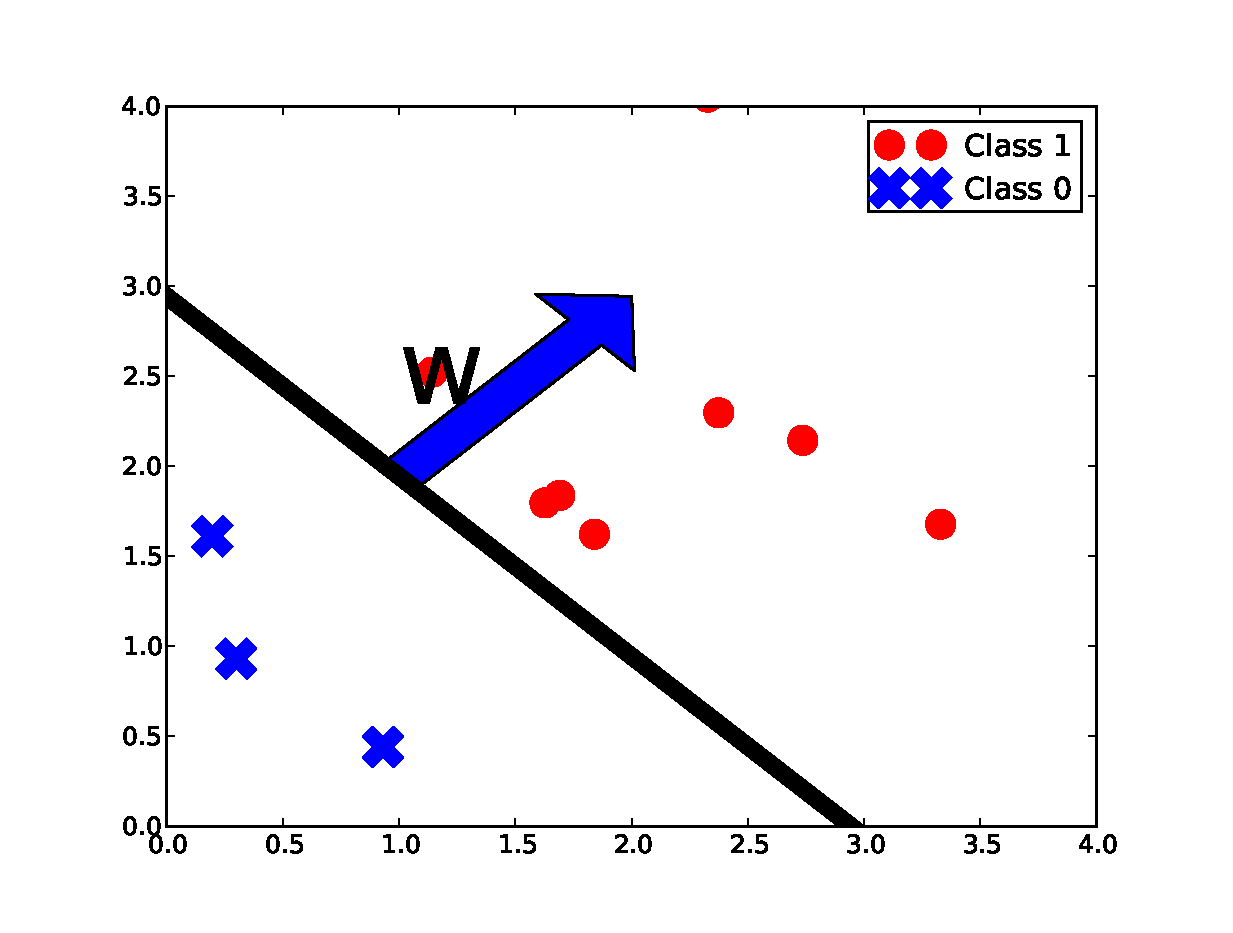
\includegraphics[width=0.7\textwidth]{../images/logistic_classifier}
  \caption{The hyperplane normal to $w$ separates space into two classes.  Whether or not this separation is correct is another story.}
\end{figure}
This happens because 
\begin{align*}
  \sigma(x\cdot w) > \delta &\quad\Leftrightarrow\quad x\cdot w > \log\frac{\delta}{1-\delta},
\end{align*}
and the set of points $x$ for which $x\cdot w$ is greater/less than some constant $c$ is the two regions on either side of the hyperplane defined by $x\cdot w = c$.  This fact is important because it is a fundamental limitation of logistic classification.  This sort of limitation is not present in other methods such as decision trees.  Note that the limitation may be a good thing if you know that the solution structure is roughly approximated by space separated by a hyperplane.  In a sense, this is a form of regularization, and prevents logistic regression from giving a ``crazy'' answer.  Also note that you are free to choose nonlinear combinations of variables, e.g. you can square some feature.  Then, in the original feature space, your separating hyperplane would be a curve.

\section{L1 regularization}
\label{logistic:section:L1}

As in section \ref{linear:section:bayesian}, we can choose a prior and form the posterior $p(w\g Y)\propto p(w)p(Y\g w)$.  As with linear regression, a Gaussian prior ($w\sim\exp{-\|w\|^2/(2\sigma_w^2)}$) is popular.  In this section we explore the consequences of choosing a Laplacian prior.  The \emph{Laplace} distribution has density function
\begin{align*}
  p(w) &\propto \exp\left( -\alpha\|w - \mu\|_1 \right), \qquad \|w\|_1 := \sum_{k=1}^K |w_k|.
\end{align*}
As with Gaussian priors, we will usually choose not to regularize the constant, and choose $\mu=0$.  In fact, we may wish to weight each term differently, in which case we will use the prior
\begin{align*}
  p(w) &= \exp\left( -\sum_{k=1}^K\alpha_k|w_k| \right), \qquad 0\leq\alpha_k<\infty.
\end{align*}
The MAP estimate is then
\begin{align}
  w_{MAP} :&= \arg\min_w\left\{ L(w) + \sum_{k=1}^K\alpha_k|w_k| \right\}.
  \label{logistic:align:map}
\end{align}
Solving for $w_{MAP}$ is known as using a Laplace prior, \emph{Lasso}, or \emph{L1 regularization}, and is related to the field of \emph{compressed sensing}.

\begin{exercise}
  Show that the MAP estimate is given by \eqref{logistic:align:map}.
\end{exercise}

As with the Gaussian MAP in linear regression, \eqref{linear:align:regularized-lsq}, the term $\sum_k\alpha_k|w_k|$ penalizes large $w$.  The effect is different in a number of ways though.  First of all, for large $|w_k|$, the $|w_k|\ll|w_k|^2$, so the penalty is smaller.  This means that the L1 regularized solution allows for larger $w_k$ than the L2 regularized solution.  Second, the optimization problem \eqref{logistic:align:map} is significantly more difficult than \eqref{linear:align:regularized-lsq} because the terms $|w_k|$ are not differentiable.  Third, and most importantly, roughly speaking, L1 regularization results in insignificant coefficients being set \emph{exactly} to zero.  This is nice because it effectively removes them from the model, which means that the effective model can be significantly simpler than in L2 regularization.  More precisely,
\begin{theorem}
  \label{logistic:theorem:L1-selection}
  With $L(w)$ the negative log likelihood given by \eqref{logistic:align:ML-soln}, suppose that the columns of the data matrix $X$ are linearly independent and that $\alpha_k>0$ for all $k$.  Then the solution $w^\ast$ to \eqref{logistic:align:map} exists and is unique.  Moreover, for every $k$, exactly one of the following holds:
  \begin{enumerate}
    \item[(i)] 
      \begin{align*}
        \left|\frac{\p L}{\p w_k}(w^\ast)\right| &= \alpha_k \quad\mbox{ and }\quad w^\ast_k\neq0
      \end{align*}
    \item[(ii)]
      \begin{align*}
        \left|\frac{\p L}{\p w_k}(w^\ast)\right| &\leq \alpha_k \quad\mbox{ and }\quad w^\ast_k=0.
      \end{align*}
  \end{enumerate}
\end{theorem}
\begin{remark}
  %Suppose we are in case (ii), then theorem \ref{logistic:theorem:L1-selection} allows for $|\p_kL(w^\ast)|$ exactly equal to $\alpha$.  However, this is a pathological case since nothing is pulling 
  This means that $\alpha_k$ sets a level at which the coefficient $k^{th}$ variable must effect the log likelihood in order for its coefficient to be nonzero.  This is contrasted with L2 regularization, which tends to result in lots of small coefficients.  This can be expected since, for small $|w_k|$, the penalty $|w_k|\gg|w_k|^2$.  In fact, one could use terms such as $|w_k|^\beta$, for $0<\beta<1$ and achieve even more sparsity.  In practice this would lead to difficulty since the problem would no longer be convex.
\end{remark}
\begin{proof}
  Since the likelihood is bounded (it is always less than one), $L(w)$ is always greater than zero.  Let $M = \max\left\{ L(w)\st |w|<1 \right\}$ and $\alpha_m:=\min\left\{ \alpha_1,\cdots,\alpha_K \right\}$.  Then, for $|w|>M/\alpha_m$ we will have 
  \begin{align*}
    L(w) + \sum_k\alpha_k|w_k| & > \sum_k\alpha_k|w_k| > \alpha_m\sum_k|w_k| > \alpha_m|w| > M.
  \end{align*}
  In other words, a local minimum must occur in the set $\left\{ w\st |w| \leq M/\alpha_m \right\}$.  Since $L$ is strictly convex, and the penalty is convex, $L(w) + \sum_k\alpha_k|w_k|$ is strictly convex and this is a global minimum and the unique solution to the optimization problem.

  The rest of the proof proceeds by linearizing $L(w)$ around the optimal point $w^\ast$.  The reader is encouraged to consider a one-dimensional problem ($w\in\Rone$) and replace $L(w)$ with $L(w^\ast) + (w-w^\ast)L'(w^\ast)$ and consider the consequences.

  Continuing with the proof, define $f(w) := L(w) + \sum_k\alpha_k|w_k|$.  Suppose that $w^\ast_k\neq0$.  Then the derivative $\p_kf(w^\ast)$ exists, and since $w^\ast$ is a minimum it must be equal to zero.  This implies (i).  To show that (ii) is a possibility, consider the function $L(w) = cw + w^2$ with $0<c\leq\alpha$ for one-dimensional $w$.  One can verify that $w^\ast=0$, and $|L'(0)| = c$, so both inequality and equality are possible.  
  
It remains to show that no situation other than (i) or (ii) is possible.  This will follow from the fact that we can never have $|\p_kL(w^\ast)| > \alpha$.  To this end, assume that $0\leq\alpha_k<c<\p_kL(w)$ (the case of negative derivative is similar).  We then have, (with $e_k$ the standard Euclidean basis vector),
\begin{align*}
  f(w + \delta e_k) &= f(w) + \delta\frac{\p L}{\p w_k}(w) \pm\delta\alpha + o(\delta)\\
  &< f(w) - \delta|c-\alpha| + o(\delta)\\
  & < f(w) \qquad\mbox{ for $\delta$ small enough}.
\end{align*}
For small enough $\delta$, we must have $f(w + \delta e_k) < f(w)$, which means $w$ is not a minimum.  This completes the proof.
\end{proof}

It should be mentioned that the problem of finding the MAP estimate \eqref{logistic:align:map} is equivalent to solving the constrained problem
\begin{align*}
  \wstar :&= \arg\min_w L(w),\qquad\mbox{subject to}\\
  \sum_{k=1}^K\alpha_k|w_k| &\leq C,
\end{align*}
for some $C$ that depends on both $\alpha$ and the function $L$.  This dependence cannot be known before solving at least one of the problems.  However, the set of values taken by the coefficients as $C$ and $\alpha$ are swept from 0 to $\infty$ (a.k.a. the \emph{path}) is the same.  Since normal cross-validation practice involves sweeping the coefficients and evaluating the models, the two methods can often be used interchangeably.

\section{Numerical solution}
\label{logistic:section:numerical}
Unlike the linear regression problem of chapter \ref{chapter:linear}, which reduced to solving a linear system, logistic regression is a nonlinear optimization problem because the \emph{objective} function (the function to be minimized) $L(w) + \sum_k\alpha_k|w_k|$ can not be reduced to solving a linear system.  In this chapter we explore iterative methods for finding a solution.  These methods give us a sequence of values $w^0,w^1,\cdots$ converging to a local minimum $\wstar$ of the objective function $f(w)$.  Each $w^j$ is found by solving a local approximation to $f$.  Note that convexity is needed to assure us that this is a global minimum.

\subsection{Gradient descent}
Perhaps the simplest method for finding a minimum of a differentiable objective function $L(w)$ is \emph{gradient descent}.  This method can be motivated by observing that, locally, a function decreases most in the direction opposite to its gradient (which is the direction of greatest local increase).  So, in our iterative search for $\wstar$, we should move in the direction opposite the gradient at our current point, see algorithm \ref{logistic:algorithm:gradient-descent} and figure \ref{logistic:figure:grad-desc}.
\begin{algorithm}
  \label{logistic:algorithm:gradient-descent}
  \caption{Gradient descent}
\begin{algorithmic}
  \State Initialize $w^0$ to some point, set $j=0$
  \State Choose $\gamma_0>0$
  \State Choose a tolerance $tol$
  \While{$err > tol$}
    \State Compute $\nabla L(w^j)$
    \State Set $w^{j+1} \gets w^j - \gamma_j\nabla L(w^j)$
    \State Set $err = |w^{j+1} - w^j|$
    \State Choose $\gamma_{j+1}$ according to some criteria
    \State Set $j\gets j+1$
  \EndWhile
\EndWhile
\end{algorithmic}
\end{algorithm}
The parameter $\gamma_j$ in algorithm \ref{logistic:algorithm:gradient-descent} can be chosen in a number of ways.  
To prevent overshooting, it is sometimes shrunk according to some criteria.  Other times, we can choose it by minimizing the one dimensional function $g(\gamma) = L(w^j - \gamma \nabla L(w^j))$.  This search is a one-dimensional optimization, and can be done using e.g. Newton's method.
\begin{figure}
  \label{logistic:figure:grad-desc}
  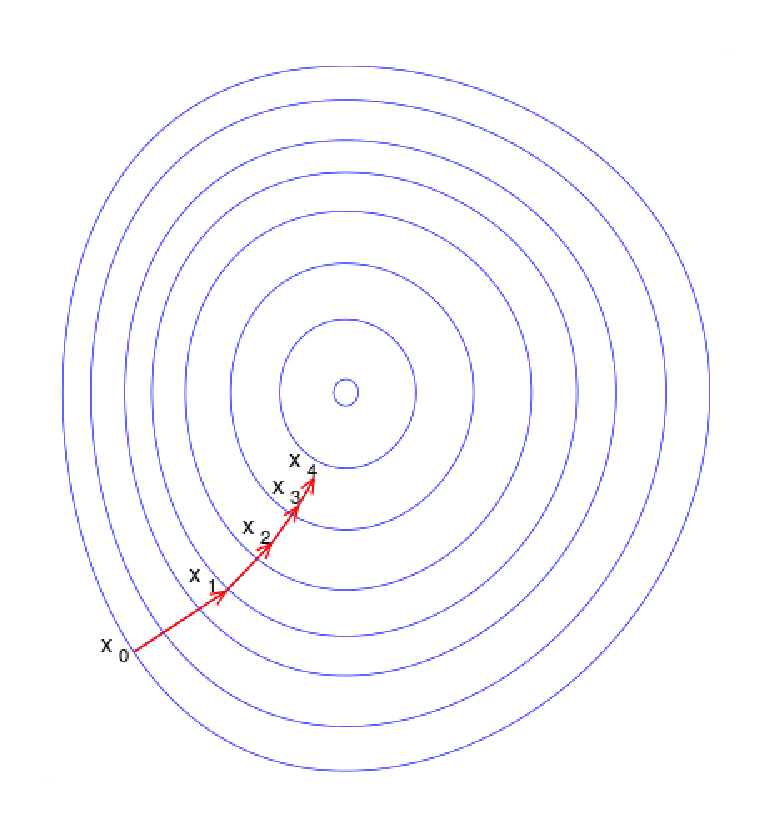
\includegraphics[width=0.5\textwidth]{../images/Gradient_descent}
  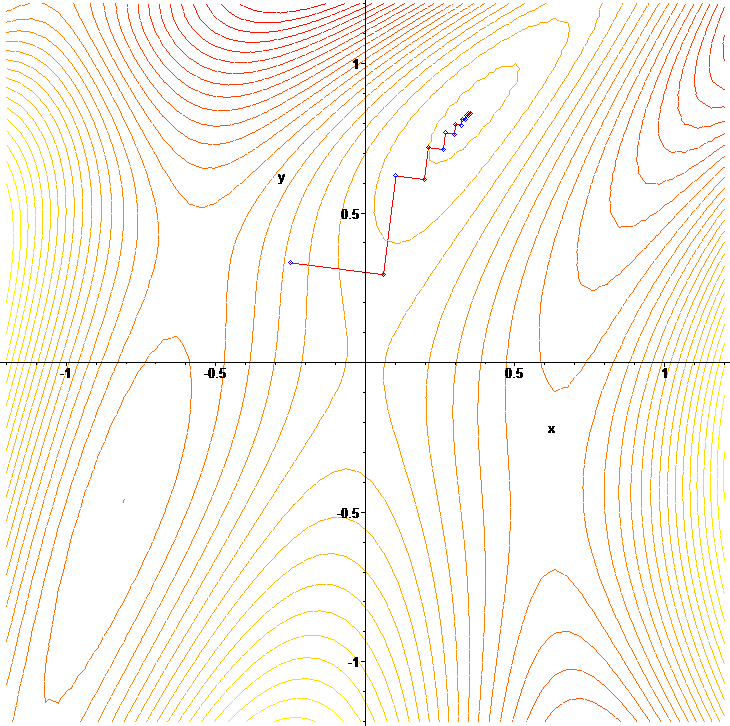
\includegraphics[width=0.5\textwidth]{../images/Gradient_descent_pathological}
  \caption{Contours show the level curves of functions.  Left:  Typical gradient descent path.  Right:  Pathological example where gradient descent zig-zags all over the place.}
\end{figure}
Gradient descent has the advantage of being very simple, and only requiring computation of the gradient.  It has the disadvantage of the fact that although the negative gradient is \emph{locally} the direction of biggest decrease in $L$, it often is not the best global direction.  In some cases, a gradient descent method can zig-zag around, missing the optimal solution, and take very long to converge.  See figure \ref{logistic:figure:grad-desc}.  Gradient descent should never be used for linear problems, since far superior methods exist here.  Another disadvantage is that it does require the gradient, which is not possible for some problems, e.g. L1 regularized regression.

\subsection{Newton's method}
For smooth objective functions where the hessian is not too difficult to compute, Newton's method is a very attractive option.  Newton's method finds zeros of functions (points where the function equals zero).   We can use Newton's method to find a minimum of $L$, since if $L$ is smooth, then at a local minimum we will have $\nabla L(\wstar)=0$.  So to optimize, we search for a zero of the gradient (and hence have to compute the hessian).  

To motivate Newton's method consider the problem of finding a zero of a one-dimensional function $g(w)$.  Suppose we are at point $w^j$ and want to find a new point $w^{j+1}$.  Approximate $g$ with the first term in its Taylor series,
\begin{align*}
  g(w) &\approx g(w^j) + (w - w^j)g'(w^j).
\end{align*}
Set this equal to zero, and get
\begin{align*}
  w^{j+1} &= w^j - \frac{g(w^j)}{g'(w^j)}.
\end{align*}
This leads to algorithm \ref{logistic:algorithm:newton-1d}
\begin{algorithm}
  \begin{algorithmic}[1]
    \caption{Newton's method for root finding (1-D)}
    \label{logistic:algorithm:newton-1d}
    \State Choose a starting point $w^0$, set $j\gets0$
    \State Choose a tolerance $tol$
    \While{$err > tol$}
        \State Compute $g'(w^j)$
        \State Set 
        \begin{align*}
          w^{j+1} &\gets w^j - \frac{g(w^j)}{g'(w^j)}.
        \end{align*}
        \State Set $err = |w^{j+1} - w^j|$
        \State Set $j\gets j+1$
    \EndWhile
  \end{algorithmic}
\end{algorithm}
In other words, at each point $w^j$, we form a linear approximation to $g(w)$, and use this to find the point at which this linear approximation is zero.

In the context of optimization, we are looking for a point where $L'(\wstar)=0$, so replace $g(w)$ with $L'(w)$ and you get the iteration step $w^{j+1} = w^j - L'(w^j)/L''(w^j)$.  In multiple dimensions, this is algorithm \ref{logistic:algorithm:newton-optimization}.
\begin{algorithm}
  \begin{algorithmic}[1]
    \caption{Newton's method for optimization}
    \label{logistic:algorithm:newton-optimization}
    \State Choose a starting point $w^0$, set $j\gets0$
    \State Choose a tolerance $tol$
    \While{$err > tol$}
        \State Compute $\nabla L(w^j)$, $\nabla^2L(w^j)$
        \State Set 
        \begin{align*}
          w^{j+1} &\gets w^j - (\nabla^2L(w^j))^{-1}\nabla L(w^j).
        \end{align*}
        \State Set $err = |w^{j+1} - w^j|$
        \State Set $j\gets j+1$
    \EndWhile
  \end{algorithmic}
\end{algorithm}

If all is well and $\nabla^2L(\wstar)$ is positive definite, then convergence to $\wstar$ is quadratic.  In this case that means $|w^{j+1}-\wstar| \leq C |w^j - \wstar|^2$ for some constant $C>0$.  If $\nabla^2L(\wstar)$ is not positive definite, then convergence can be very slow.  This, along with the need to compute and invert the hessian, are the major drawbacks of Newton's method for optimization.

\subsection{Solving the $L1$ regularized problem}
While gradient descent and Newton's method are available for maximum likelihood estimation, the L1 regularized problem requires special care (since it isn't smooth).  One technique (of many) is to transform the our MAP problem (which is unconstrained, and nonsmooth in $K$ unknowns)
\begin{align}
  \label{logistic:align:L1-again}
  \wstar :&= \arg\min_w \left\{ L(w) + \sum_{k=1}^K\alpha_k|w_k| \right\}
\end{align}
to the equivalent constrained, smooth problem in $2K$ unknowns
\begin{align}
  \label{logistic:align:L1-reformulated}
  \begin{split}
    (\wstar, \ustar) :&= \arg\min\left\{ L(w) + \sum_{k=1}^K\alpha_ku_k \right\},\\
    \mbox{subject to: }& -u_k\leq w_k \leq u_k,\qquad k=1,\cdots,K.
  \end{split}
\end{align}
Of course we don't care about the ``dummy'' variables $\ustar$, and they can be thrown away once the problem is done (they should equal $|w_k|$ at the minimum).

\begin{exercise}
  Show that if $(\wstar, \ustar)$ is a solution to \eqref{logistic:align:L1-reformulated}, then $\wstar$ is also a solution to \eqref{logistic:align:L1-again}.  
\end{exercise}

To solve \eqref{logistic:align:L1-reformulated}, a variety of approaches can be taken.  Since the objective function has at least two continuous derivatives, it is possible to replace it with a quadratic approximation (keep the first two terms in a Taylor series), get a best guess, then iterate.  This is the same goals as Newton's method, except here we have to deal with constraints.  A discussion of how this is done is beyond the scope of this text.

\subsection{Common numerical issues}
Here we discuss common numerical issues encountered when solving the maximum likelihood problem \eqref{logistic:align:ML-soln}.

\emph{Perfect separation} occurs when some hyperplane perfectly separates $\RK$ into one region where all training points have label 0, and another region where training points have label 1.  As an example, consider a one-dimensional logistic regression where we have two training data points:

\begin{tabular}{|l|r|}
  \hline
  X & Y \\
  \hline
  -1 & 0 \\
  \hline
  1 & 1 \\
  \hline
\end{tabular}

Before we write any equations, what do you think will happen?  Remember that this is not a Bayesian model, and it tries to fit the training data as well as it can.  From the model's perspective, it thinks that if $x=-1$, then $y$ will \underline{always} be zero!  Moreover, if $x=1$, the model thinks $y$ will always be 1.  What will our model say about the other points?  As it turns out, the maximum likelihood solution is $w=\infty$ (if you can call this a solution, since no computer will ever reach this point), and the model will say that any negative point $x$ will correspond to $y=0$ with 100\% certainty, and that any positive point $x$ will correspond to $y=1$ with 100\% certainty.
\begin{exercise}
  Consider a logistic regression problem with training data as above.  Note that we will not use a constant in this model.  
  \begin{enumerate}
    \item Show that for any $w\in\Rone$, $L(w+1)< L(w)$, and that as $w\to\infty$, $L(w)$ decreases to $0$.  This means that the maximum likelihood ``solution'' is $w_{ML}=\infty$.
    \item Show that this could not happen if you used $L1$ or $L2$ regularization.
    \item Draw the function $\sigma(x\cdot w)$ for $w = 10000000$, and $x\in[-3, 3]$.
    \item What is a separating hyperplane for this problem?
  \end{enumerate}
\end{exercise}

When perfect separation occurs, the numerical solution cannot converge.  A good solver will detect that $|w|\to\infty$ and will give you a warning.  The question for the modeler is, ``what to do next?''  It is possible that you included too many variables, since, if you have as many variables as you have data points (and all data points are unique), then you will always be able to find a separating hyperplane.  In this case, it makes sense to remove variables or increase the number of data points.

The next issue is specific to Newton's method.  Recall the expression for the hessian \eqref{logistic:align:grad-hess} and the discussion following it.  This showed that if there is linear dependency in the columns of $X$, then the hessian will be singular.  This will cause an error in Newton's method.  What to do?  You could regularize, which would eliminate this error.  You could also switch to a solver that did not require inversion of the hessian.  Our viewpoint however is that a singular hessian points to redundancy in the data, and that finding and eliminating that redundancy should be the first priority.  This can be done by eliminating columns from $X$ and checking if the rank of $X$ does not change.  If it does not change, then that column was redundant.
%Recall that, roughly speaking, Newton's method approximates $L(w) \approx L(\wstar) + \nabla L(\wstar) + \nabla^2L(\wstar)$, and solves for the minimum of this quadratic approximation.  

%The first Newton method specific issue is that, if there is linear dependency in the columns of $X$, then $\nabla^2L(w)$ will be singular for all $w$.  To make this plausible, consider the case where the first and second columns are exactly the same.  Since $L$ depends on $w_1$ and $w_2$ only through the algebraic term $w_1X_{n1} + w_2X_{n2} = (w_1 + w_2)X_{n1}$, changes in $w$ that preserve the term $w_1 + w_2$ make no difference.  Since these changes make no difference in $L$, they cannot possibly make a difference in $\nabla^2L$, which implies that $\nabla^2L$ will be singular.

%The second Newton method specific issue is slightly more subtle.  Suppose the first independent variable has absolutely no effect on $y$.  In this case, we do not expect $L$ to change when we change $w_1$, and therefore the first row and column of $\nabla^2L$ will be all zeros, which in turn implies that $\nabla^2L$ will be singular.  Of course, just by luck, changing $w_1$ will change $L$ a little bit, but this change will be very small when $N$ is large, and therefore $\nabla^2L$ will almost be singular.  A similar problem happens if two columns are almost the same, except for some noise that is unrelated to $y$.

\section{Model evaluation}

Linear regression can be thought of as a classifier that produces a probability of class inclusion.  This is no different than a Naive Bayes estimator, and the methods of section \ref{classification:subsection:roc} are applicable.  In particular, ROC curves are commonly used.  

The negative log likelihood is another candidate for measuring the goodness of fit.  The first difficulty arising with using the negative log likelihood is that it will increase in magnitude at a rate proportional to $N$.  This means we cannot hope to compare $L(w)$ for different size data sets. We can deal with this by dividing by $N$, giving the \emph{normalized negative log likelihood} $N^{-1}L$.  This is a good candidate to compare different models for the \emph{same} problem.  In other words, we can add/subtract variables and see how it effects $N^{-1}L$.  We can also compare $N^{-1}L$ in the training and test/cross-validation sets.

The normalized negative log likelihood $N^{-1}L$ does however depend quite a bit on the ``difficulty'' of the problem, and generally is not interpretable from problem to problem.  For this reason, it is usually not a meaningful quantity to share with people.  An alternative is the so-called (McFadden's) pseudo R-sqared,
\begin{align*}
  \Psi R2 :&= 1 - \frac{L(\wstar)}{L_{null}(\wstar)},
\end{align*}
where $L_{null}$ is the negative log likelihood obtained by using a model with \emph{only} a constant (the \emph{null model}).  Inspection of the definition reveals that $\Psi R2$ measures how much our full model improves on the null model.  Also, like $R$ squared, $0\leq\Psi R2\leq 1$.  Moreover, just like in linear regression, the ratio $L/L_{null}$ is the ratio of the negative log likelihoods.  This means that McFadden's pseudo R-squared is a generalization of $R^2$ from linear regression.  See bullet point (ii) below \eqref{linear:align:R2}.

\begin{exercise}
  Suppose your boss says, ``just figure out the R-square of your logistic regression model in the exact same way as you do for linear regression.''  Tell your boss why this is impossible.
\end{exercise}

\begin{exercise}
  Assume our ``full model'' (the one giving rise to $L$) is built with a constant and other variables.  Show that the in-sample $\Psi R2$ is between zero and one, with both zero and one as possible values.
\end{exercise}

\section{End Notes}

A great introduction to convex optimization has been written by Boyd and Vandenberghe.  It focuses on problem formulation and is hence applicable for users of the algorithms. \cite{BoydConvexOpt}.
